% -----------------------------------------------------------------------
% KNOSYS submission — Knowledge-Based Systems (Elsevier)
% Template: elsarticle
% Review: Single-blind (author info required — no anonymization needed)
% References: natbib + elsarticle-num.bst (numbered/Vancouver)
% Compile: pdflatex → bibtex → pdflatex → pdflatex
% -----------------------------------------------------------------------
\documentclass[preprint,12pt]{elsarticle}

% -----------------------------------------------------------------------
% Packages
% -----------------------------------------------------------------------
\usepackage{natbib}
\usepackage{graphicx}
\usepackage{booktabs}
\usepackage{array}
\usepackage{multirow}
\usepackage{amsmath}
\usepackage{amssymb}
\usepackage{microtype}
\usepackage{url}
\usepackage{hyperref}
\usepackage{xcolor}
\usepackage{amsthm}
\usepackage{tikz}
\usetikzlibrary{shapes.geometric,arrows.meta,positioning,calc,fit,backgrounds}

\newtheorem{remark}{Remark}

% -----------------------------------------------------------------------
% Convenience macros
% -----------------------------------------------------------------------
\newcommand{\vtot}{V_{\text{total}}}
\newcommand{\cone}{V_1}
\newcommand{\ctwo}{V_2}
\newcommand{\cthree}{V_3}
\newcommand{\ka}{Krippendorff's~$\alpha$}
\newcommand{\fk}{Fleiss'~$\kappa$}
\newcommand{\ck}{Cohen's~$\kappa$}
\newcommand{\icc}{\text{ICC}(A,1)}

\journal{Knowledge-Based Systems}

% -----------------------------------------------------------------------
\begin{document}

\begin{frontmatter}

\title{Measurement Without Validity: The Compounding Reliability Problem in Agentic AI Evaluation}


\author[addr1]{William Caban\corref{cor1}}
\ead{wcabanba@redhat.com}

\cortext[cor1]{Corresponding author. ORCID: 0009-0008-1211-7050}

\address[addr1]{Red Hat, Inc., Raleigh, North Carolina, USA;
  Alma Mater Europaea University, Vienna, Austria}

% -----------------------------------------------------------------------
\begin{abstract}
Agentic AI evaluation pipelines produce benchmark scores that justify deployment
decisions, safety certifications, and regulatory compliance claims. No formal
framework has yet characterized how validity degrades across the stages of these
pipelines. We present a three-layer compounding validity model,
$V_{\text{total}} \leq V_1 \times V_2 \times V_3$, that captures multiplicative
degradation across task generation ($V_1$), human-simulator calibration ($V_2$),
and automated judgment ($V_3$). Under empirically grounded estimates, a pipeline
retaining 70\% validity at each stage is at most 34\% valid against the intended
construct (range~0.22--0.54).

We validate the model against a structured survey of 55 published agentic
evaluation papers, finding that approximately 82\% apply structurally mismatched,
incomplete, or absent inter-rater reliability (IRR) metrics---a pattern consistent
with systematic $V_3$ collapse. We further identify empirical evidence of $V_1$
failures (task validity flaws in 7 of 10 popular benchmarks) and $V_2$
miscalibration (up to 9 percentage points inter-simulator variance, with systematic
demographic disparities for non-Standard American English speakers).

We derive eight prescriptions grounded in psychometric science and domain-stratified
reliability thresholds (ICC$\geq$0.70; $\alpha \geq 0.67$/$0.70$/$0.80$ by
consequence level) that practitioners and benchmark authors can apply immediately.
The framework provides a tractable knowledge-based tool for diagnosing and
correcting evaluation pipeline validity before deployment decisions are made.
\end{abstract}

\begin{keyword}
inter-rater reliability \sep agentic AI evaluation \sep construct validity \sep
LLM-as-a-Judge \sep knowledge-based evaluation framework \sep decision support \sep
benchmark quality
\end{keyword}

\end{frontmatter}

% -----------------------------------------------------------------------
\section{Introduction}
\label{sec:intro}

Deployment decisions, safety certifications, and regulatory compliance claims for
agentic AI systems are all downstream of a number that appears deceptively clean: a
benchmark score. That score is the product of a pipeline (task generation, world
simulation, rater judgment), and each stage of that pipeline is a potential source of
systematic, non-random measurement error.

The measurement problem in agentic evaluation is not simply that individual
components are imperfect. It is that the imperfections compound. A pipeline that
loses 30\% of valid signal at task generation, 20\% at simulation, and 25\% at the
judgment layer does not produce evaluation that is 75\% valid. Under the most
optimistic independence assumption, it produces evaluation that retains less than
42\% of valid signal against the intended construct. Under correlated failures (which
are more likely), it is worse.

This paper makes three contributions. First, we document empirically that agentic
evaluation fails three distinct psychometric validity tests simultaneously, and that
the empirical evidence for each failure is published, peer-reviewed, and specific.
Second, we formalize the three-layer compounding validity model and show that failures
multiply rather than add---a relationship the field has not yet quantified. Third, we
derive eight prescriptions from the psychometric literature that practitioners and
benchmark authors can apply immediately.

We are not arguing that agentic evaluation is worthless. We are arguing that it is
less valid than current practices acknowledge, that the mechanisms of invalidity are
known, and that the standards for reporting and interpreting evaluation results should
be substantially higher.

% -----------------------------------------------------------------------
\section{Background: The Psychometric Standard}
\label{sec:background}

This section introduces the two psychometric constructs that underpin the analysis:
construct validity, which defines what a measurement system is supposed to capture,
and inter-rater reliability, which quantifies the consistency of the scoring process.
Both are necessary conditions for a valid benchmark score.

\subsection{Construct Validity as the Organizing Concept}
\label{sec:construct-validity}

The foundational criterion for any measurement system is construct validity: whether
the measurement instrument actually captures the phenomenon it claims to measure
\citep{cronbach1955}. The measurement science tradition identifies three evaluable
validity types that together constitute evidence for or against construct validity:

\begin{itemize}
  \item \textbf{Content validity}: does the evaluation cover the full scope of the
    construct, or only an easily measurable subset? Does a benchmark described as
    ``measuring agentic tool use'' sample the full range of tool-use behaviors, or
    does it measure only the subset most amenable to automated scoring (e.g., API call
    success rate)?
  \item \textbf{Criterion validity} (concurrent and predictive): does the evaluation
    score correlate with an external criterion of the target construct? Predictive
    criterion validity specifically asks whether the score predicts real-world
    deployment performance.
  \item \textbf{Construct validity evidence} (convergent and discriminant): does the
    evaluation correlate with conceptually related measures (convergent evidence) and
    fail to correlate with conceptually unrelated ones (discriminant evidence)?
\end{itemize}

Despite its centrality to measurement science, construct validity has received
limited attention in AI evaluation, even as benchmark creation involves numerous
high-stakes design decisions including target user selection,
construct-to-task operationalization, and scoring metric choice \citep{liu2024}. A
systematic review of 84 academic and industry papers found that technical performance
was represented in 83\% of evaluated works, while human-centered evaluation appeared
in only 30\%, and both were combined in only 15\% \citep{meimandi2025}. Benchmark
success and deployment value remain systematically disconnected.

Content validity failures are measurable and consequential. A systematic analysis of
194,955 benchmark questions mapped against the EU~AI~Act's taxonomy of model
capabilities found that current benchmarks devote 61.6\% of regulatory-relevant
coverage to hallucination tendency and 31.2\% to performance reliability, while
capabilities central to loss-of-control scenarios (including evading human oversight,
self-replication, and autonomous AI development) receive zero coverage across the
entire public benchmark corpus \citep{prandi2025}.

\subsection{Inter-Rater Reliability: Metrics and Their Conditions of Use}
\label{sec:irr-metrics}

Inter-rater reliability (IRR) quantifies the degree to which raters (human
annotators, LLM judges, or Agent-as-a-Judge systems) agree on the same outcome.
The appropriate IRR metric is determined by the structure of the rating design, not
by convention or familiarity.

\textbf{\ck} \citep{cohen1960} is appropriate when exactly two fixed raters score
every item using the same two-rater configuration across all items. It corrects for
chance agreement using per-rater marginal distributions.

\textbf{\fk} \citep{fleiss1971} generalizes to three or more raters, with the
critical property that rater identity may vary per item provided the number of
ratings per item is constant. It uses the pooled distribution across all raters for
its chance-agreement correction. This is the correct metric for fixed-size judge
panels where individual judge identity may rotate.

\textbf{\ka} \citep{krippendorff2004} is the most general metric: it handles any
number of raters with varying identity, supports missing data natively, and
accommodates nominal, ordinal, interval, and continuous measurement scales through
interchangeable distance functions. For ordinal rubrics, it uses ranked distance
rather than binary mismatch, correctly weighting the severity of disagreement.

\textbf{Intraclass Correlation Coefficient (ICC)} extends IRR concepts to
continuous outcomes. The two-way mixed-effects absolute agreement form,
$\text{ICC}(A,1)$, measures the degree to which scores from one rater (or
measurement occasion) agree in absolute value with scores from another. Unlike
$\kappa$-family metrics, $\text{ICC}(A,1)$ is appropriate when outcomes are
measured on a continuous or interval scale and when absolute agreement (not merely
consistency of ranking) is the validity target. In the context of this paper, it
is used to quantify simulation calibration: the agreement between agent success
rates under simulated versus real user conditions ($V_2$, Section~\ref{sec:layer2}).

Table~\ref{tab:irr-selection} summarizes metric selection by scenario.

\begin{table}[ht]
\centering
\caption{IRR metric selection by agentic evaluation scenario.}
\label{tab:irr-selection}
\small
\begin{tabular}{@{}p{0.38\linewidth}p{0.25\linewidth}p{0.28\linewidth}@{}}
\toprule
Scenario & Recommended metric & Reason \\
\midrule
3+ LLM judges, binary, complete matrix
  & \fk & Nominal data, complete, multi-rater \\[4pt]
3+ LLM judges, 1--5 rubric, complete matrix
  & \ka{} (ordinal) & Ordinal distance metric needed \\[4pt]
Crowdsourced annotation with missing ratings
  & \ka & Handles missingness natively \\[4pt]
2 human annotators, categorical labels
  & \ck & Only valid two-rater case \\[4pt]
Continuous scores from LLM judges
  & \ka{} (interval) & Interval distance required \\[4pt]
Rotating judge panel membership per task
  & \ka & Varying rater identity; possible missingness \\
\bottomrule
\end{tabular}
\end{table}

\subsection{Reliability Thresholds and Their Origins}
\label{sec:thresholds}

The Landis--Koch scale \citep{landis1977} is the most frequently cited threshold
system in AI evaluation: $\kappa > 0.21$ as ``fair,'' $\kappa > 0.41$ as
``moderate,'' $\kappa > 0.61$ as ``substantial.'' This scale was developed for
behavioral science contexts with human raters and has no special authority in AI
evaluation. Its widespread use as an acceptability benchmark for LLM judge agreement
is a category error.

For agentic evaluation, domain-calibrated thresholds grounded in construct validity
theory are more appropriate. We propose the following tiered thresholds, derived in
Section~\ref{sec:prescriptions}:

\begin{itemize}
  \item \textbf{Exploratory capability evaluation}: $\alpha \geq 0.67$
    \citep[pp.~241--243]{krippendorff2004}
  \item \textbf{Safety, bias, fairness, and risk scoring}: $\alpha \geq 0.70$
    (\emph{proposed; see Prescription~5})
  \item \textbf{Scoring that gates deployment, compliance, or regulatory reporting}:
    $\alpha \geq 0.80$ (\emph{proposed; see Prescription~5})
\end{itemize}

% -----------------------------------------------------------------------
\section{Related Work}
\label{sec:related}

\subsection{Evaluation Documentation and Knowledge Frameworks}

Structured knowledge frameworks for AI evaluation documentation have emerged as a
response to inconsistent reporting practices. \citet{mitchell2019} introduced Model
Cards, encoding expert knowledge about model behavior, intended use, and limitations
into a standardized artifact that practitioners can apply without deep ML expertise.
\citet{dhar2025} extended this to Evaluation Disclosure Cards (EvalCards), providing
a structured template that enforces reporting of evaluation methodology, including IRR
and construct validity criteria. These frameworks follow the knowledge-based systems
tradition of encoding expert domain knowledge into structured decision procedures that
non-specialists can apply consistently \citep{hayes1983,buchanan1984}: just as early
medical expert systems (MYCIN, INTERNIST) encoded diagnostic knowledge into rule-based
structures, documentation frameworks encode evaluation methodology expertise into
required reporting fields. The compounding validity model ($\vtot \leq V_1 \times V_2
\times V_3$) and the IRR metric selection decision tree proposed in this paper
complement these documentation standards by providing the underlying validity model
that determines \emph{what} to report before documentation is written.

\subsection{Validity Theory Applied to AI Evaluation}

The foundational measurement science concept this paper applies is construct
validity \citep{cronbach1955}: whether a measurement instrument captures the
phenomenon it claims to measure. Despite its centrality, construct validity has
received limited attention in AI evaluation practice \citep{liu2024}.
\citet{jacobs2021} demonstrated that fairness metrics routinely measure constructs
different from their stated targets---a specific instance of the construct validity
failure this paper formalizes at the pipeline level. \citet{meimandi2025} provided
empirical evidence that agentic AI evaluation systematically fails to support the
productivity claims it is used to justify, a finding consistent with the $V_1$
failures documented in Section~\ref{sec:layer1}. The three-layer compounding model
operationalizes construct validity theory for multi-stage automated pipelines,
providing a tractable computational framework for what has previously been treated
as a qualitative concern.

\subsection{Decision Support for Reliability Metric Selection}

The IRR metric selection decision tree (Figure~\ref{fig:decision-tree}) follows the
expert system tradition of encoding domain expertise into formal decision procedures
that practitioners can apply without deep methodological background
\citep{krippendorff2004}. \citet{james2026} provided a systematic guide to
inter-annotator agreement metric selection in NLP annotation, arguing against
one-size-fits-all use of Cohen's $\kappa$---a position directly aligned with the
prescriptions in Section~\ref{sec:prescriptions}. The decision tree proposed here
extends this guidance to agentic AI evaluation pipelines, encoding the structural
conditions (rater count, identity stability, measurement scale) that determine metric
validity into a formal procedure. This knowledge representation is the framework's
primary deployable artifact: it transforms implicit expert knowledge about IRR metric
selection into an explicit, auditable decision structure.

% -----------------------------------------------------------------------
\section{Layer 1: Task Generation Validity}
\label{sec:layer1}

In traditional static benchmarks, tasks and ground truth are fixed. Reliability can
be validated once against a stable reference. In agentic evaluation, tasks are often
dynamically generated by language models, embedding systematic biases from the
generator into the evaluation distribution before a single agent response is scored.

The construct validity problem at this layer is that dynamically generated tasks may
not sample the intended construct uniformly. An LLM task generator that
overrepresents certain task types, difficulty levels, or surface forms creates a
distribution that raters can agree on perfectly, while measuring something
systematically different from the intended capability.

The empirical evidence is specific. A study evaluating 10 popular agentic benchmarks
found task validity flaws in 7 of them and outcome validity flaws in 7 of them, with
all 10 showing benchmark reporting gaps \citep{zhu2025}. Documented failures include
task validity failures where do-nothing agents passed 38\% of airline booking tasks,
and outcome validity failures where LLM judges made arithmetic errors. Every benchmark
showed at least one validity failure category; none provided sufficient evidence to
support unqualified capability claims.

Task generation validity must be assessed before any IRR analysis is meaningful. A
rating matrix derived from systematically biased tasks cannot be rescued by metric
sophistication at the judgment layer.

% -----------------------------------------------------------------------
\section{Layer 2: Simulation Calibration}
\label{sec:layer2}

Many agentic benchmarks evaluate agents in interaction with simulated users or
simulated world environments rather than real humans and real environments. This
design choice is operationally sensible (real human interaction at evaluation scale
is expensive and slow), but it introduces a second, distinct validity problem:
whether the simulated environment faithfully proxies the real deployment context.

\subsection{Empirical Evidence of Simulation Miscalibration}
\label{sec:sim-evidence}

The most direct empirical evidence comes from \citet{seshadri2026}, which tested
LLM user simulation against real human users on $\tau$-Bench retail tasks across
participants in the United States, India, Kenya, and Nigeria. The findings establish
simulation miscalibration as a measured fact rather than a theoretical concern:

\begin{itemize}
  \item Agent success rates varied up to 9 percentage points across different LLM
    user simulators, demonstrating that simulation results are not robust to
    simulator choice.
  \item Evaluations using simulated users exhibited systematic directional
    miscalibration: underestimating agent performance on challenging tasks while
    overestimating it on moderately difficult ones.
  \item Simulated users introduced conversational artifacts absent from real
    interactions: elevated question-asking, heightened politeness markers, and
    artificial turn structures.
\end{itemize}

\subsection{The Demographic Asymmetry Problem}
\label{sec:demographic}

The calibration failures documented by \citet{seshadri2026} are not uniformly
distributed across user populations. African American Vernacular English (AAVE)
speakers experienced consistently worse success rates and calibration errors than
Standard American English (SAE) speakers, with disparities compounding with age.
Indian English speakers showed similar patterns.

This is simultaneously a measurement validity failure and a fairness failure. An
evaluation pipeline calibrated on SAE simulated users is not a valid measurement of
agentic capability for AAVE-speaking or non-SAE users. As shown in Section~\ref{sec:layer3},
the same demographic asymmetry is compounded at the judgment layer by LLM judges that
exhibit systematic miscalibration across dialect groups independently of simulation
layer failures.

\subsection{Why Agreement on a Distorted Signal Does Not Establish Measurement Validity}
\label{sec:distorted-signal}

The key inferential step at this layer is often missed: high rater agreement on
simulated interactions does not demonstrate evaluation reliability. It demonstrates
that all raters agree on a distorted input.

A scoring panel that perfectly agrees on agent scores produced by an
AAVE-miscalibrated simulator has achieved high IRR in the technical sense. It has
also produced a high-reliability measurement of the wrong thing. Agreement on a
distorted signal is agreement on distortion.

% -----------------------------------------------------------------------
\section{Layer 3: Metric Misspecification}
\label{sec:layer3}

The third layer of validity failure occurs at judgment: even when a human or LLM
judge scores agent outputs, the inter-rater reliability metric used to validate that
scoring is structurally mismatched to the pipeline design in the large majority of
published evaluations.

\subsection{Why \ck{} Is Structurally Wrong for Most Agentic Evaluation Designs}
\label{sec:cohen-kappa}

\ck{} requires exactly two raters scoring every item, with the same two-rater pair
maintained across all items. Almost no agentic evaluation design satisfies this
constraint:

\begin{itemize}
  \item LLM-as-a-Judge pipelines typically use a rotating pool of judge models that
    vary across evaluation runs or item subsets.
  \item Agent-as-a-Judge frameworks \citep{zhuge2025} explicitly assign different
    agent-judges per task type, domain, or stakeholder persona.
  \item Human annotation at scale uses crowdsourcing pools where rater identity
    varies per item.
  \item Dynamic benchmark generation produces item batches scored by different
    annotator subsets.
\end{itemize}

Applying \ck{} to any of these designs produces a mathematically invalid result,
because its chance-agreement correction assumes fixed rater identity. Using it
anyway (common in practice) is a silent validity failure that produces an
uncorrectable reliability estimate without warning.

\subsection{The Literature Scan: IRR in Published Agentic Evaluation Papers}
\label{sec:scan}

\textit{Methodology.} We conducted a structured survey of 55 papers published or
posted between 2022 and 2026, selected via a stratified purposive approach across
nine topic categories: major agentic benchmarks; automated grader validity studies;
benchmarks with correct IRR use; LLM-as-a-Judge studies; benchmarks with structural
metric mismatch; long-horizon evaluation; safety and RLHF annotation; recent
2025--2026 evaluation papers; and safety-critical IRR failure cases. Within each
category, papers were selected for citation prominence, venue tier (ACL, EMNLP,
NeurIPS, ICLR), and direct relevance to evaluation methodology; arXiv preprints in
cs.AI and cs.CL supplemented peer-reviewed coverage where thin. This is a purposive
stratified survey, not a systematic review: the sample is designed to cover the main
failure modes rather than to exhaust a keyword-defined corpus.

Coding was applied against four pre-specified dimensions: (1)~the IRR metric reported
or absent, (2)~the rater design (number of raters, fixed or rotating identity),
(3)~the measurement scale (binary, nominal, ordinal, or continuous), and (4)~whether
the metric's structural assumptions were satisfied by the pipeline design.
The full coding criteria are documented in Appendix~\ref{app:literature}.

\textit{Reliability validation.} Coding was performed by the primary author. To
assess coding reliability, a stratified random sample of $N=20$ papers (36\% of the
corpus, proportionally allocated across the nine topic categories) was coded
independently by three LLM raters from distinct model families: NVIDIA
Nemotron-Ultra-550B, Google Gemma-4-31B, and Alibaba Qwen3-80B-A3B
\citep{openrouter2026}. Each LLM rater
received only the coding instrument and the paper's abstract and evaluation
methodology passage, with no access to the primary-rater codes. Four-way
Krippendorff's~$\alpha$ across the author and all three LLM raters for the
structural validity dimension was $\alpha = 0.89$ (pairwise range: $0.86$--$0.93$),
meeting the exploratory reliability threshold of $\alpha \geq 0.67$ adopted in the
prescriptions of this paper.

\textit{Finding ($\alpha = 0.89$; four-rater validation).} Across 55 coded papers,
approximately 10 (18\%) appear to use structurally correct IRR metrics with explicit
rationale. The remaining 45 exhibit one of three failure modes:

\paragraph{Mode 1: Automated Grading, No IRR (11\%).}
Major benchmark papers---$\tau$-bench \citep{yao2024}, \textsc{OSWorld} \citep{xie2024},
\textsc{SWE-bench} \citep{jimenez2024}, \textsc{GAIA} \citep{mialon2024}, and
\textsc{WebArena} \citep{zhou2024webarena}---use deterministic automated graders or
unvalidated LLM judges with no IRR measurement against human annotation; $\tau^2$-Bench
\citep{barres2025}, the quality-fix follow-up to $\tau$-bench, takes the same approach:
tighter automated grading rather than human IRR validation. \citet{gurram2026} directly
measures the gap: substring-based automated evaluation achieves $\kappa = 0.049$ against
human annotation (essentially chance-level) while a three-LLM ensemble achieves only
$\kappa = 0.432$. The Verified re-releases of these benchmarks
(\textsc{WebArena Verified}, \citealt{elhattami2025}: Cohen's $\kappa = 0.83$)
demonstrate that rigorous human annotation produces fundamentally different reliability
evidence.

\paragraph{Mode 2: Structural Metric Mismatch (16\%).}
Papers that do report IRR most commonly apply \ck{} to panels of three or more LLM
judges, or report raw percentage agreement for ordinal and ternary scales without
chance correction (\citealt{fan2026} AgentProcessBench: 89.1\% on ternary labels).
In \citet{han2025} the mismatch is more subtle: \ck{} is applied as a series of
pairwise comparisons (each of 54 LLMs vs.\ human ratings), each individually a valid
two-rater design, but the results are then aggregated and interpreted as panel
reliability across 54 configurations with varying rater compositions, a use case
requiring \fk{} or \ka, not repeated two-rater $\kappa$.

\paragraph{Mode 3: Wrong Metric for the Measurement Construct (31\%).}
Safety, preference, and RLHF papers apply metrics appropriate for one statistical
question to answer a different one: Pearson correlation for ordinal safety ratings
from 112 demographically diverse annotators \citep{movva2024}; ELO ratings
substituting for inter-annotator reliability in crowdsourced pairwise preference
\citep{chiang2024}; raw percent agreement without chance correction for 40
contractors ranking model outputs \citep[72--77\%]{ouyang2022}.

\paragraph{Mode 4: No Metric Reported (24\%).}
The largest single category by paper count (13 of 55) reports no IRR metric of any
kind. This group includes RLHF annotation pipelines, red-teaming studies, and safety
evaluation reports in which the absence of reliability reporting is treated as
unremarkable. Unlike Mode~1 (automated graders that could in principle be validated
against human annotation), Mode~4 papers lack sufficient information to even assess
which metric would be appropriate. The absence of any reliability report is a
complete $V_3$ validity gap.

Table~\ref{tab:failure-modes} summarizes the distribution.

\begin{table}[ht]
\centering
\caption{IRR failure modes across 55 coded papers. Only 10 (18\%) use structurally
correct metrics with explicit rationale.}
\label{tab:failure-modes}
\small
\begin{tabular}{@{}p{0.30\linewidth}rr>{\raggedright\arraybackslash}p{0.42\linewidth}@{}}
\toprule
Failure mode & Papers & \% & Representative example \\
\midrule
Automated grading, no IRR         & 6  & 11 & $\tau$-bench, \textsc{OSWorld}, \textsc{SWE-bench} \\
Structural metric mismatch        & 9  & 16 & \ck{} for 54-LLM panel \citep{han2025} \\
Wrong construct / \% only         & 17 & 31 & InstructGPT; Chatbot Arena (ELO) \\
No metric reported                & 13 & 24 & RLHF pipelines, Red Teaming \\
\textbf{Correct metric}           & \textbf{10} & \textbf{18} & \textsc{WebArena Verified} ($\kappa = 0.83$) \\
\bottomrule
\end{tabular}
\end{table}

\textit{Structural contrast.} The 10 papers using IRR correctly share a
distinguishing behavior: they report multiple metrics explicitly and state their
rationale. Papers using incorrect metrics report only \ck{} with no structural
justification. The mismatch is not a deliberate simplification; it reflects
unawareness of the structural conditions that govern metric validity.

\subsection{Demographic Asymmetry in LLM Judge Calibration}
\label{sec:judge-demographic}

The metric mismatch problem documented above is compounded by a systematic calibration
asymmetry in LLM judges across linguistic varieties. In a study evaluating three LLMs
as toxicity judges across 60 language varieties spanning 10 language clusters,
LLM--human agreement was the weakest dimension of consistency---weaker than
cross-model or cross-dialect consistency---with systematic gaps across dialectal
groups \citep{faisal2024}. Judge miscalibration for non-standard dialect speakers
persists in direct LLM judgment, independently of the simulation layer failures
documented in Section~\ref{sec:demographic}.

The implication for the compounding model is asymmetric $V_3$: benchmarks using LLM
judges without dialect-stratified calibration validation will produce $V_3$ values
that overstate validity for SAE-speaker user populations and understate it for
non-SAE populations. This is an IRR validity failure that structurally correct metric
selection cannot by itself correct, because the miscalibration occurs within the
judge's learned behavior, not in the choice of metric.

\subsection{Ordinal Rubrics and the Kappa Penalty}
\label{sec:kappa-penalty}

Most agentic evaluation rubrics use ordinal scoring (e.g., 1--5 on helpfulness,
safety, coherence). \fk{} treats all disagreements as categorically equal: a rater
scoring 1 when others score 5 is penalized identically to a rater scoring 4 when
others score 5. This is wrong for ordinal data.

The consequence is bidirectional distortion: \ck{} and \fk{} artificially inflate
apparent disagreement when raters are closely aligned on an ordinal scale (one point
apart) and can underestimate disagreement when raters are at opposite ends of the
scale. For safety evaluation, this matters: a safety rubric where judges disagree by
1 point appears as unreliable as one where they disagree by 4 points.

\subsection{Metric Selection Decision Tree}
\label{sec:decision-tree}

Figure~\ref{fig:decision-tree} provides a decision tree for selecting the
structurally correct IRR metric based on rater design, data completeness, and
measurement scale.

\begin{figure}[t]
\centering
\begin{minipage}[t]{0.65\linewidth}%
\resizebox{\linewidth}{!}{%
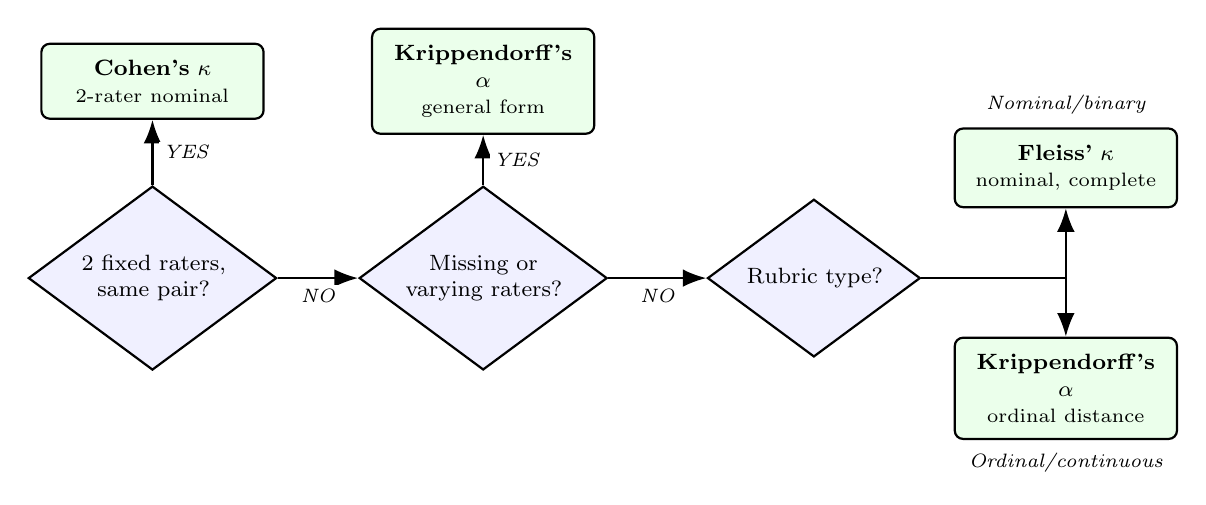
\begin{tikzpicture}[
  baseline=(CK.north),
  dec/.style={diamond, draw, thick, fill=blue!6, text width=2.2cm,
              align=center, inner sep=1pt, aspect=1.35, font=\footnotesize},
  term/.style={rectangle, draw, thick, fill=green!8, rounded corners=3pt,
               text width=2.4cm, align=center, minimum height=0.9cm,
               inner sep=6pt, font=\footnotesize},
  arr/.style={-{Latex[length=3mm]}, thick},
  lbl/.style={font=\scriptsize\itshape, fill=white, inner sep=1.5pt}
]
\node[dec] (Q1) at (0,   0) {2 fixed raters, same pair?};
\node[dec] (Q2) at (4.2, 0) {Missing or varying raters?};
\node[dec] (Q3) at (8.4, 0) {Rubric type?};
\node[term] (CK)    at (0,   2.5) {\textbf{Cohen's $\kappa$}\\{\scriptsize 2-rater nominal}};
\node[term] (KAgen) at (4.2, 2.5) {\textbf{Krippendorff's $\alpha$}\\{\scriptsize general form}};
\node[term] (FK)    at (11.6,  1.4) {\textbf{Fleiss' $\kappa$}\\{\scriptsize nominal, complete}};
\node[term] (KAord) at (11.6, -1.4) {\textbf{Krippendorff's $\alpha$}\\{\scriptsize ordinal distance}};
\draw[arr] (Q1.east) -- node[lbl, below=2pt]{NO} (Q2.west);
\draw[arr] (Q2.east) -- node[lbl, below=2pt]{NO} (Q3.west);
\draw[arr] (Q1.north) -- node[lbl, right=2pt]{YES} (CK.south);
\draw[arr] (Q2.north) -- node[lbl, right=2pt]{YES} (KAgen.south);
\coordinate (forkX) at (FK.south |- Q3.east);
\draw[thick] (Q3.east) -- (forkX);
\draw[arr]   (forkX)   -- (FK.south);
\draw[arr]   (forkX)   -- (KAord.north);
\node[lbl, above=3pt, align=center] at (FK.north)    {Nominal/binary};
\node[lbl, below=3pt, align=center] at (KAord.south) {Ordinal/continuous};
\end{tikzpicture}%
}%
\end{minipage}%
\hfill%
\begin{minipage}[t]{0.30\linewidth}%
\scriptsize
\textbf{Selection rules:}
\medskip

\noindent\textbf{Cohen's $\kappa$}\\
Exactly 2 fixed raters, same pair, every item.
\medskip

\noindent\textbf{Fleiss' $\kappa$}\\
$\geq$3 raters, complete matrix, nominal/binary rubric.
\medskip

\noindent\textbf{Krippendorff's $\alpha$} (general)\\
Missing ratings or rater identity varies.
\medskip

\noindent\textbf{Krippendorff's $\alpha$} (ordinal)\\
Complete matrix; ordinal or continuous rubric.
\medskip

{\tiny\itshape Using \ck{} outside the 2-rater
fixed-pair case produces an invalid reliability
estimate without warning.}
\end{minipage}
\caption{IRR metric selection. Left: decision tree based on rater design, matrix
completeness, and rubric scale. Right: selection rules summary. Using \ck{} outside
the two-rater fixed-pair case is a silent validity failure.}
\label{fig:decision-tree}
\end{figure}

Figure~\ref{fig:decision-tree} is a knowledge-based decision support system in the
expert systems tradition~\citep{james2026}: it encodes domain expert knowledge about
IRR metric structural assumptions into a formal decision procedure that practitioners
can apply without background in psychometrics. The four decision nodes correspond to
the four structural conditions that govern metric validity; the terminal nodes are
executable recommendations. A practitioner who provides the rater count, identity
stability, and scale type obtains a structurally correct metric recommendation without
needing to understand the mathematical foundations of chance-agreement correction.
This procedural knowledge representation is the framework's primary deployable
artifact, complementing the governance prescriptions in Section~\ref{sec:prescriptions}.

% -----------------------------------------------------------------------
\section{The Compounding Argument}
\label{sec:compounding}

The full mathematical derivation, including the correlated-failure extension and a
practical estimation protocol, is in Section~\ref{sec:applying} and
Appendix~\ref{app:compounding}.

\subsection{Formal Statement}
\label{sec:formal}

Let $\cone \in [0,1]$ denote the task generation validity: the degree to which the
generated task distribution matches the ideal construct distribution, defined as one
minus the total variation distance between them. Because the ideal construct
distribution $D_{\mathcal{C}^*}$ is a theoretical object and not directly observable,
$\cone$ cannot be computed from first principles; in practice it is estimated by
comparing generated tasks against a curated expert reference set
(Appendix~\ref{app:compounding}, \S{}B.6). Let $\ctwo \in [0,1]$ denote the
simulation calibration validity, defined as the $\icc$ between simulated and real
agent outcomes on a matched task set, estimated separately per user population group.
Let $\cthree \in [0,1]$ denote the judgment validity: the appropriate IRR metric
value (\ka{} or \fk, per the pipeline's measurement scale) for the rating design.

The overall construct validity of the evaluation pipeline is bounded above by:
\begin{equation}
  \vtot \leq \cone \times \ctwo \times \cthree
  \label{eq:bound}
\end{equation}

The bound holds under the assumption of independence between layer failures. When
layer failures are positively correlated (as they are likely to be when the same
provider family operates at all three layers), $\vtot$ falls below this bound. The
independence assumption is therefore optimistic; the correlated-failure bound is
tighter (Appendix~\ref{app:compounding}, \S{}B.4).

Figure~\ref{fig:pipeline} illustrates the three-layer pipeline with its validity
estimates and the compounding formula.

\begin{figure}[t]
\centering
\resizebox{\textwidth}{!}{%
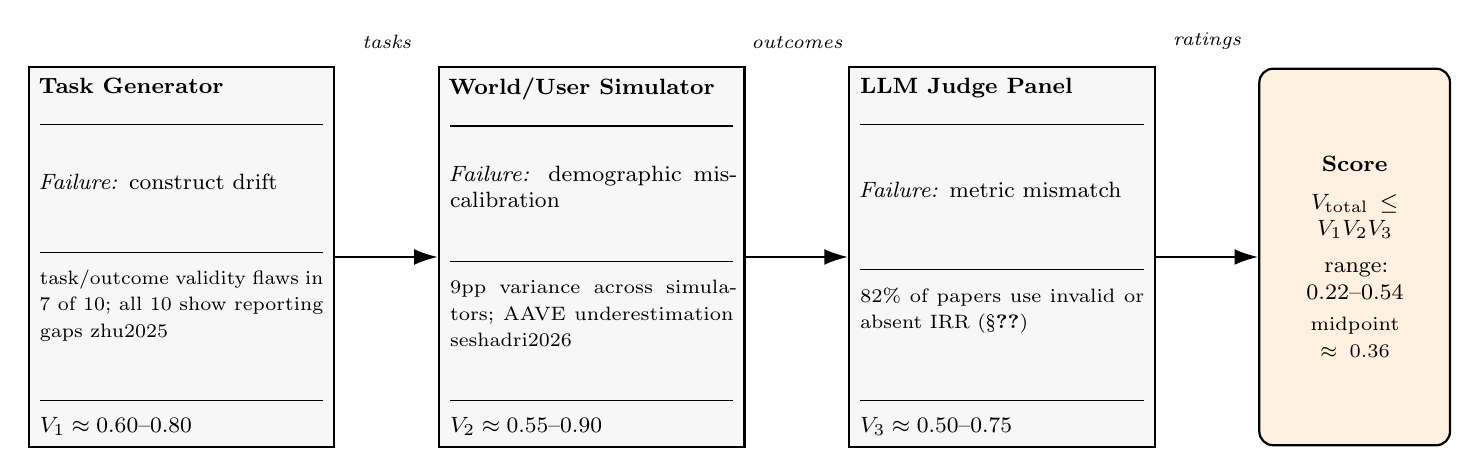
\begin{tikzpicture}[
  layer/.style={rectangle, draw, thick, fill=gray!6, inner sep=4pt, font=\footnotesize},
  score/.style={rectangle, draw, thick, fill=orange!12, text width=2.0cm,
                align=center, minimum height=4.782cm, rounded corners=5pt,
                inner sep=6pt, font=\footnotesize},
  arr/.style={-{Latex[length=3mm, width=2mm]}, thick},
  lbl/.style={font=\scriptsize\itshape, fill=white, inner sep=2pt}
]
\node[layer] (G) {%
  \parbox[t][4.5cm][s]{3.6cm}{%
    \textbf{Task Generator}\\[2pt]%
    \rule{3.6cm}{0.5pt}%
    \vfill%
    \textit{Failure:} construct drift%
    \vfill%
    \rule{3.6cm}{0.3pt}\\[2pt]%
    {\scriptsize task/outcome validity flaws in 7 of 10; all 10 show reporting gaps \citep{zhu2025}}%
    \vfill%
    \rule{3.6cm}{0.3pt}\\[2pt]%
    $V_1 \approx 0.60$--$0.80$%
  }%
};
\node[layer, right=1.3cm of G] (S) {%
  \parbox[t][4.5cm][s]{3.6cm}{%
    \textbf{World/User Simulator}\\[2pt]%
    \rule{3.6cm}{0.5pt}%
    \vfill%
    \textit{Failure:} demographic miscalibration%
    \vfill%
    \rule{3.6cm}{0.3pt}\\[2pt]%
    {\scriptsize 9pp variance across simulators; AAVE underestimation \citep{seshadri2026}}%
    \vfill%
    \rule{3.6cm}{0.3pt}\\[2pt]%
    $V_2 \approx 0.55$--$0.90$%
  }%
};
\node[layer, right=1.3cm of S] (J) {%
  \parbox[t][4.5cm][s]{3.6cm}{%
    \textbf{LLM Judge Panel}\\[2pt]%
    \rule{3.6cm}{0.5pt}%
    \vfill%
    \textit{Failure:} metric mismatch%
    \vfill%
    \rule{3.6cm}{0.3pt}\\[2pt]%
    {\scriptsize 82\% of papers use invalid or absent IRR (\S\ref{sec:scan})}%
    \vfill%
    \rule{3.6cm}{0.3pt}\\[2pt]%
    $V_3 \approx 0.50$--$0.75$%
  }%
};
\node[score, right=1.3cm of J] (SC) {%
  \textbf{Score}\\[4pt]%
  $\vtot \leq V_1 V_2 V_3$\\[4pt]%
  range: 0.22--0.54\\[2pt]%
  {\scriptsize midpoint $\approx 0.36$}%
};
\draw[arr] (G.east) -- (S.west);
\draw[arr] (S.east) -- (J.west);
\draw[arr] (J.east) -- (SC.west);
\node[lbl, above=4pt] at ($(G.north east)!0.5!(S.north west)$)  {\itshape tasks};
\node[lbl, above=4pt] at ($(S.north east)!0.5!(J.north west)$)  {\itshape outcomes};
\node[lbl, above=4pt] at ($(J.north east)!0.5!(SC.north west)$) {\itshape ratings};
\end{tikzpicture}%
}%
\caption{Three-layer agentic evaluation pipeline with validity estimates. Each layer
introduces a distinct failure; failures compound multiplicatively under the
independence bound ($\vtot \leq V_1 \times V_2 \times V_3$, range $0.22$--$0.54$,
midpoint $\approx 0.36$). The bound tightens further under correlated failures when
the same model family operates at all three layers.}
\label{fig:pipeline}
\end{figure}

\subsection{Applying the Model to Published Benchmarks}
\label{sec:worked-example}

Table~\ref{tab:vtotal} applies the compounding model to six widely-used agentic
benchmarks using values drawn directly from the cited literature.

\textbf{$V_1$ sources}: \citet{zhu2025} identified task validity failures
per benchmark: do-nothing agents passed 38\% of $\tau$-bench airline tasks
($V_1 = 0.62$); stale CSS caused 28\% performance underestimation in OSWorld
($V_1 = 0.72$); augmented test cases changed 41\% of SWE-bench rankings
($V_1 = 0.59$); WebArena's LLM judge introduced 1.6--5.2\% misestimation
($V_1 = 0.97$).

\textbf{$V_2$ sources}: OSWorld, SWE-bench, and WebArena use real computer or web
environments without LLM user simulators; $V_2 = 1.00$ for these.
For $\tau$-bench, \citet{seshadri2026} measured Expected Calibration Error
($\mathrm{ECE}_{\mathrm{Human-LLM}}$) between simulated and real user outcomes.
We operationalize $V_2 \approx 1 - \mathrm{ECE}/100$: 11.7\% for Standard American
English speakers ($V_2 = 0.88$) and 20.3\% for AAVE speakers ($V_2 = 0.80$).

\textbf{$V_3$ sources}: For benchmarks with no reported human IRR, we use the
empirically measured automated grader validity from \citet{gurram2026}: substring
matching achieves $\kappa = 0.049$ against human annotation on comparable tasks
(chance-level). This is the empirical V3 floor for automated-only evaluation.
For WebArena Verified, $V_3 = 0.83$ from the reported Cohen's $\kappa$ between two
fixed human annotators \citep{elhattami2025}.

\begin{table}[ht]
\centering
\caption{Compounding validity bounds for published agentic benchmarks, using
values derived from the cited literature. $V_3^*$: no IRR reported; value estimated
from automated grader validity against human annotation (Gurram 2026, $\kappa=0.049$).
$V_2^{\dagger}$: real environment, no LLM user simulator.}
\label{tab:vtotal}
\small
\begin{tabular}{@{}lcccc@{}}
\toprule
Benchmark & $V_1$ & $V_2$ & $V_3$ & $\vtot \leq$ \\
\midrule
$\tau$-bench retail (SAE users) & 0.62 & 0.88 & 0.05$^*$ & \textbf{0.027} \\
$\tau$-bench retail (AAVE users) & 0.62 & 0.80 & 0.05$^*$ & \textbf{0.025} \\
OSWorld & 0.72 & 1.00$^{\dagger}$ & 0.05$^*$ & \textbf{0.036} \\
SWE-bench & 0.59 & 1.00$^{\dagger}$ & 0.05$^*$ & \textbf{0.030} \\
WebArena (original) & 0.97 & 1.00$^{\dagger}$ & 0.05$^*$ & \textbf{0.049} \\
WebArena Verified & 0.97 & 1.00$^{\dagger}$ & 0.83 & \textbf{0.805} \\
\bottomrule
\end{tabular}
\end{table}

Three findings emerge. First, every benchmark without human IRR ($V_3 \approx 0.05$)
produces $\vtot < 0.05$ regardless of $V_1$ and $V_2$: less than 5\% of valid signal
survives the judgment layer alone. The automated grader is the binding constraint.

Second, correcting $V_3$ through rigorous human annotation increases $\vtot$ by
approximately 16$\times$: WebArena original ($\vtot \leq 0.049$) versus WebArena
Verified ($\vtot \leq 0.805$). The only difference is the addition of two fixed
human annotators with $\kappa = 0.83$. This demonstrates empirically that
Prescription~2 (metric selection) and Prescription~8 (IRR as a required reporting
field) are the highest-leverage interventions.

Third, the demographic disparity documented by \citet{seshadri2026} appears in $V_2$
(SAE: 0.88 vs.\ AAVE: 0.80) but produces similarly low $\vtot$ for both groups
(0.027 vs.\ 0.025) because $V_3 = 0.05$ dominates. For populations where $V_3$ is
corrected, the $V_2$ gap becomes the binding constraint and the fairness
implications are larger.

\subsection{Implications for Published Benchmark Claims}
\label{sec:implications}

When a paper reports that ``Agent X achieves 82\% on [benchmark],'' the epistemic
weight of that claim is conditioned on the validity of the three pipeline layers.
Under the compounding model, an 82\% score from a benchmark with $\vtot \leq 0.049$
(Table~\ref{tab:vtotal}, WebArena original) does not tell us that the agent achieves
82\% of the intended capability. It tells us that the agent achieves some unknown
capability level, measured by an instrument that retains less than 5\% of valid
signal against the intended construct.

This does not mean the score is uninformative. It means its interpretation requires
the three validity layers to be assessed and reported alongside the score. The
WebArena Verified result ($\vtot \leq 0.805$) demonstrates that this standard is
achievable at the cost of adding rigorous human IRR to the evaluation design.

% -----------------------------------------------------------------------
\section{Prescriptions for Valid Agentic Evaluation}
\label{sec:prescriptions}

Items supported by existing literature are stated as requirements; items that extend
beyond current literature are marked \emph{we propose}.

\begin{enumerate}

\item \textbf{Validate simulation calibration before trusting evaluation results.}
Use a held-out set of real human interactions to measure the $\icc$ between simulated
and real agent outcomes. If calibration is not validated, the evaluation signal is of
unknown reliability regardless of how precisely the judging rubric is specified
\citep{seshadri2026}. Report the calibration ICC alongside any benchmark result that
uses user simulation. \emph{We propose $\icc \geq 0.70$ as a minimum threshold for
simulation calibration, set 3pp above \citet{krippendorff2004}'s general content
analysis minimum of 0.67 because LLM simulators exhibit systematic behavioral
artifacts absent from trained-human rater contexts \citep{seshadri2026}.}

\item \textbf{Select the IRR metric based on pipeline structure, not convention.}
Apply \ck{} only when exactly two fixed raters score every item. Apply \fk{} when a
fixed-size panel of three or more raters scores nominal or categorical outcomes on a
complete matrix. Apply \ka{} when the rubric is ordinal or continuous, when missing
ratings are possible, or when rater panel membership varies. Using \ck{} outside its
structural assumptions is a silent validity failure (Section~\ref{sec:layer3}).

\item \textbf{Report both \fk{} and \ka{} for any rubric using ordinal or interval
scales.} When the two metrics diverge, the divergence is itself diagnostic:
$\kappa < \alpha$ suggests raters are frequently one scale point apart rather than at
opposite ends of the range, a much healthier disagreement pattern than the $\kappa$
score alone would imply.

\item \textbf{Use cross-family judge ensembles.} Self-preference and family-level
bias in LLM judges \citep{spiliopoulou2025,wataoka2024} are large enough to distort
comparative agent rankings. Evaluation pipelines should use judges from at least two
distinct provider families and report inter-judge agreement across families.
Single-family judge panels produce spuriously inflated within-family agreement.

\item \textbf{Apply domain-appropriate reliability thresholds.}
For exploratory capability evaluation, $\alpha \geq 0.67$ is the minimum consistent
with \citet[pp.~241--243]{krippendorff2004}'s own recommendation. For safety, bias,
fairness, and risk scoring, \emph{we propose} $\alpha \geq 0.70$. For scoring that
gates model deployment, compliance certification, or regulatory reporting, \emph{we
propose} $\alpha \geq 0.80$. When these thresholds cannot be met, as \citet{jafari2026}
demonstrate for LLM mental health response evaluation (three certified psychiatrists
produced $\text{ICC} = 0.087$--$0.295$ and $\alpha = -0.203$), the correct response
is not to lower the threshold but to recognize that the construct is insufficiently
specified for reliable measurement.

\item \textbf{Validate dynamically generated task distributions against curated
reference sets.} When tasks are generated by an LLM, validate that the generated
distribution samples the intended construct by testing a sample of generated tasks
against domain-expert judgment: present tasks to experts who rate each on whether it
faithfully instantiates the target construct, and compute $V_1$ as the proportion
rated as construct-valid \citep{zhu2025}. Where a curated expert reference set
exists, total variation distance between the generated and reference distributions
provides a more formal measure; in practice, expert-rated proportions are the
tractable operationalization (Section~\ref{sec:applying}, Step~1).

\item \textbf{Stratify evaluation by demographic and linguistic group.} Simulation
calibration failures are not uniformly distributed across user populations
\citep{seshadri2026}, and LLM judge calibration failures show the same pattern across
dialect groups \citep{faisal2024}. AAVE speakers, Indian English speakers, and other
non-SAE populations must be included in calibration validation before benchmark
results are considered representative.

\item \textbf{Report IRR as a required field in evaluation documentation.}
Standardized reporting frameworks such as \textsc{EvalCards} \citep{dhar2025} provide
the infrastructure to enforce consistent disclosure across papers and model releases.
Including IRR metric, threshold, and metric-selection rationale as required fields
in evaluation reporting cards would institutionalize the prescriptions above at the
submission level.

\end{enumerate}

% -----------------------------------------------------------------------
\section{Applying the Framework: A Pipeline Assessment Procedure}
\label{sec:applying}

The following procedure operationalizes the compounding validity model as a
knowledge-based pipeline assessment tool. Pipeline operators can apply it at
evaluation design time to estimate $\vtot$ and identify which layer requires the most
attention before results are reported.

\begin{enumerate}

\item \textbf{Estimate $V_1$ (task generation validity).} Generate a sample of 100
  tasks from the pipeline's task generator $G$. Present them to domain experts who
  score each task on whether it faithfully samples the intended construct. Compute
  $V_1$ as the proportion rated as construct-valid. If a curated reference set is
  available, measure total variation distance between generated and reference
  distributions instead.

\item \textbf{Estimate $V_2$ (simulation calibration).} Run a matched subset of
  tasks (minimum 50) with both the LLM simulator $S$ and real human users. Compute
  $\mathrm{ICC}(A,1)$ between simulated and real agent success rates, separately for
  at least two user population groups (e.g., SAE and one non-SAE group). Use the
  population-weighted average as $V_2$.

\item \textbf{Estimate $V_3$ (judgment validity).} Apply the IRR metric selection
  procedure (Figure~\ref{fig:decision-tree}) to identify the structurally correct
  metric for the pipeline's rater design. Compute that metric on a sample of ratings.
  This value is $V_3$.

\item \textbf{Compute the bound.} $\vtot \leq V_1 \times V_2 \times V_3$. Report
  this bound alongside any benchmark result derived from the pipeline.

\end{enumerate}

\noindent\textbf{Interpretation guideline.} If $\vtot \leq 0.50$, benchmark scores
should not be used for consequential deployment decisions without independent
validation. If $\vtot \leq 0.30$, the pipeline should be redesigned before any
deployment claim is made. The formal derivation and correlated-failure extension
are in Appendix~\ref{app:compounding}.

% -----------------------------------------------------------------------
\section{Threats to Validity}
\label{sec:threats}

We assess threats to the validity of this study following the construct, internal,
external, and conclusion validity framework standard in empirical research methodology
\citep{wohlin2012,jedlitschka2008}.

\subsection{Construct Validity}
\label{sec:construct-threats}

\textit{Operationalization of $V_1$, $V_2$, $V_3$.} The three validity measures are
operationalizations of theoretical constructs. The ideal construct distribution
$D_{\mathcal{C}^*}$ (Section~\ref{sec:formal}) is a theoretical object; $V_1$
cannot be computed from first principles and is estimated here from published
benchmark failure rates \citep{zhu2025} rather than direct total variation distance
measurement. $V_2$ is operationalized via Expected Calibration Error (ECE) rather
than ICC$(A,1)$: specifically, $V_2 \approx 1 - \mathrm{ECE}_{\mathrm{Human-LLM}}/100$
from \citet{seshadri2026}. This is an approximation; the equivalence holds only when
ECE measures uniform miscalibration, which is not guaranteed. $V_3$ for benchmarks
without human IRR uses the automated grader validity floor ($\kappa = 0.049$) from
\citet{gurram2026} rather than a direct IRR measurement for each specific benchmark.
Readers should treat the values in Table~\ref{tab:vtotal} as derived estimates
rather than direct measurements of each construct.

\textit{IRR coding taxonomy.} The four-dimension coding scheme
(Section~\ref{sec:scan}) may not capture all relevant failure modes. In particular,
papers that apply the structurally correct metric but with an incorrect threshold, or
that report IRR on a subset of items not representative of the full evaluation, fall
outside the coding scheme and may be classified as ``correct'' when they should not
be. Appendix~\ref{app:literature} provides the full coding table to support
independent assessment.

\textit{Compounding model.}
The multiplicative validity bound (Equation~\ref{eq:bound}) is presented as a
conceptual model, explicitly not a proved theorem (Appendix~\ref{app:compounding},
\S{}B.3). The motivating argument assumes layer independence and treats each $V_i$
as a normalized signal-to-noise ratio; both assumptions are approximations. The bound
should be read as a formalization of the compounding intuition, not a mathematical
guarantee.

\subsection{Internal Validity}
\label{sec:internal-threats}

\textit{Coding reliability.} The literature scan (Section~\ref{sec:scan}) was coded
by the primary author. To address the potential self-referential tension (a paper about
IRR using single-rater coding), we conducted a four-rater reliability study on a
stratified $N=20$ subsample. Three LLMs from distinct model families (NVIDIA
Nemotron-Ultra-550B, Google Gemma-4-31B, Alibaba Qwen3-80B-A3B;
\citealt{openrouter2026}) independently applied the coding instrument to the same
excerpts, with no access to the primary-rater codes.
Four-way Krippendorff's~$\alpha = 0.89$ on the structural validity dimension meets the
paper's own exploratory threshold ($\alpha \geq 0.67$), supporting the 82\% IRR misuse
prevalence as an IRR-validated finding rather than a structured estimate.

A secondary tension is worth naming explicitly: this paper argues that LLMs exhibit
systematic miscalibration as evaluative raters (Sections~\ref{sec:demographic}
and~\ref{sec:layer3}), yet uses LLM raters as a validation mechanism here. These are
not equivalent roles. The $\alpha = 0.89$ result does not claim that LLMs are
valid substitutes for domain-expert human raters; it demonstrates that the coding
instrument is sufficiently unambiguous to be applied consistently by raters from
different model families, none of whom had access to the author's codes. Instrument
clarity (can independent agents apply the same decision rules?) is a more limited
claim than rater validity (do the raters' judgments track the true construct?), and
it is the former that the four-rater study supports. The
pre-specified coding criteria and full coding table in Appendix~\ref{app:literature}
make individual coding decisions verifiable independently by human readers.

\textit{Purposive sampling and confirmation bias.} The 55-paper sample was selected
purposively to cover nine topic categories, not to exhaust a keyword-defined corpus.
This exposes the scan to selection bias: papers demonstrating failures may be more
visible (cited more, identified more easily) than papers with correct but unreported
IRR practices. The author's prior belief that IRR is systematically misused may have
influenced which papers were included in each category or how ambiguous cases were
coded. The structured category definitions and transparent category membership
(Appendix~\ref{app:literature}) mitigate but do not eliminate this threat.

\subsection{External Validity}
\label{sec:external-threats}

\textit{Sample scope.} The 55 papers were drawn primarily from English-language
venues (ACL, EMNLP, NeurIPS, ICLR) and arXiv preprints in cs.AI and cs.CL. Papers
from other geographic regions, language communities, or non-English venues may show
different IRR reporting patterns. The temporal scope (2022--2026) means that earlier
work and work after the scan cutoff is not captured; IRR practices are evolving and
the field may improve.

\textit{Domain of the compounding model.} The three-layer model was constructed for
agentic evaluation pipelines involving task generation, user simulation, and LLM
judgment. Static benchmarks with fixed tasks, no simulation layer, and human-only
raters present a different threat model where only Layer~3 (IRR metric selection)
directly applies. The prescriptions in Section~\ref{sec:prescriptions} are intended
to generalize across evaluation pipeline designs, but their applicability to static
benchmarks should be assessed separately.

\subsection{Conclusion Validity}
\label{sec:conclusion-threats}

\textit{Independence assumption.} The primary conclusion of Section~\ref{sec:compounding}
is that validity failures compound multiplicatively. This conclusion depends on the
independence assumption: that layer failures are statistically unrelated. When the
same underlying mechanism (e.g., the same LLM provider family) operates at all three
layers, failures are positively correlated and $\vtot$ falls below the independence
bound. The conclusion is therefore stated conservatively: the independence bound is
presented as optimistic, and correlated-failure scenarios are shown to produce lower
$\vtot$ (Appendix~\ref{app:compounding}, \S{}B.4). The qualitative conclusion
(failures multiply rather than add) is robust to the independence assumption because
the bound holds as an upper limit regardless of correlation structure.

\textit{Derived estimates in Table~\ref{tab:vtotal}.} The $V_i$ values in the
benchmark table (Section~\ref{sec:worked-example}) are derived from published
measurements using approximations documented in the construct validity subsection
above. The $V_3$ floor ($\kappa = 0.049$) is drawn from a single study
\citep{gurram2026} on one task type; whether it generalizes to deterministic
automated graders (e.g., test-suite execution in SWE-bench) or other evaluation
designs is an open empirical question.

To bound the sensitivity of the primary conclusion to this assumption, Table~\ref{tab:sensitivity}
shows $\vtot$ across three $V_3$ scenarios for the $\tau$-bench and SWE-bench cases.

\begin{table}[ht]
\centering
\caption{Sensitivity of $\vtot$ to $V_3$ assumption for two representative benchmarks.
$V_1$ and $V_2$ values are held fixed at the values in Table~\ref{tab:vtotal}.
$V_3 = 0.05$ is the automated grader floor from \citet{gurram2026};
$V_3 = 0.30$ and $V_3 = 0.50$ represent plausible scenarios for higher-quality
automated graders.}
\label{tab:sensitivity}
\small
\begin{tabular}{@{}lcccc@{}}
\toprule
Benchmark & $V_1$ & $V_2$ & $V_3$ & $\vtot \leq$ \\
\midrule
$\tau$-bench retail (SAE) & 0.62 & 0.88 & 0.05 & \textbf{0.027} \\
$\tau$-bench retail (SAE) & 0.62 & 0.88 & 0.30 & \textbf{0.164} \\
$\tau$-bench retail (SAE) & 0.62 & 0.88 & 0.50 & \textbf{0.274} \\
\midrule
SWE-bench & 0.59 & 1.00 & 0.05 & \textbf{0.030} \\
SWE-bench & 0.59 & 1.00 & 0.30 & \textbf{0.177} \\
SWE-bench & 0.59 & 1.00 & 0.50 & \textbf{0.295} \\
\bottomrule
\end{tabular}
\end{table}

Even under the most optimistic $V_3 = 0.50$ scenario, $\vtot$ remains below 0.30
for both benchmarks, falling below the pipeline-redesign threshold proposed in
Section~\ref{sec:applying}. The qualitative conclusion (benchmarks without human IRR
validation retain less than 30\% of valid signal even under generous assumptions)
is robust across the full $V_3$ sensitivity range. A reader who assigns $V_3 > 0.50$
to automated graders is implicitly claiming that automated grading achieves moderate
reliability against human annotation on these specific benchmark tasks; that claim
should be supported by direct grader-vs-human measurement analogous to
\citet{gurram2026}, which has not been published for these benchmarks.

% -----------------------------------------------------------------------
\section{Discussion}
\label{sec:discussion}

\subsection{What This Paper Does Not Claim}
\label{sec:not-claim}

We do not claim that current agentic evaluations are worthless. They provide
directional signal. We claim that the field's current practices overstate the
validity and precision of that signal, and that the standards for reporting should be
substantially higher. A benchmark result reported without IRR metrics, simulation
calibration evidence, and metric selection justification is incomplete, in the same
way that a clinical measurement reported without instrument validity data is
incomplete.

\subsection{The Governance Stakes}
\label{sec:governance}

For academic benchmark comparisons, validity limitations are a scientific quality
issue. For deployment decisions, safety certifications, and regulatory claims, they
are a governance failure. Agentic AI systems are increasingly being deployed in
consequential contexts. The evaluation apparatus used to justify those deployments
must meet the same validity standards applied to any measurement-driven governance
process.

The regulatory dimension makes this concrete. Emerging frameworks such as the EU~AI
Act require evidence of comprehensive risk assessment for general-purpose AI models.
A systematic analysis of 194,955 benchmark questions found that capabilities central
to loss-of-control (including evading human oversight, self-replication, and
autonomous AI development) receive zero benchmark coverage \citep{prandi2025}. If
the construct coverage gap means that no existing benchmark can provide evidence of
regulatory compliance, then the IRR validity of those benchmarks is a secondary
concern: the primary problem is that they do not measure what regulations require.
Both failures must be addressed together.

\subsection{Broader Impact}
\label{sec:broader-impact}

This work raises the evidential bar for deployment certifications, surfaces
demographic calibration failures that existing evaluation practice obscures, and
gives practitioners eight actionable criteria they can apply using existing
psychometric tools.

Three misuse risks follow from this work. First, the proposed reliability thresholds
($\alpha \geq 0.70$, $\alpha \geq 0.80$) may become compliance checkboxes rather
than genuine validity indicators. Meeting a threshold does not guarantee valid
measurement; it establishes the minimum condition for a score to be interpretable.
Second, stratified calibration across demographic and linguistic groups increases
evaluation cost; benchmark maintainers and shared evaluation platforms should bear
primary responsibility for calibration coverage, not individual research teams.
Third, the finding that three certified psychiatrists produced $\text{ICC} =
0.087$--$0.295$ on LLM mental health safety evaluation \citep{jafari2026} should not
discourage research in high-stakes AI domains. It means the construct is
underspecified for reliable measurement, which calls for more rigorous construct
development, not withdrawal.

% -----------------------------------------------------------------------
\section{Conclusion}
\label{sec:conclusion}

The move from static to dynamic agentic evaluation does not reduce the importance of
inter-rater reliability; it multiplies the surfaces on which reliability can fail
and introduces new systematic biases at each layer: task generation, world
simulation, and judgment. The compounding effect means that an evaluation pipeline
with moderate validity problems at each of three layers can produce an evaluation
signal that is far less valid than any single-layer estimate would suggest.

The science of measurement was not built for static benchmarks alone. It was built
for situations where the measurement apparatus is a source of variance, where raters
disagree in structured rather than random ways, and where the construct must be
separated from the instrument measuring it. That is agentic evaluation.

These standards are achievable. \citet{elhattami2025} (\textsc{WebArena Verified})
demonstrates this directly: adding rigorous human annotation with two fixed annotators
and reporting Cohen's $\kappa = 0.83$ [0.81, 0.85] satisfies the metric selection
requirement (Prescription~2), exceeds the exploratory reliability threshold
(Prescription~5), and treats IRR as a required reporting field (Prescription~8).
\textsc{WebArena Verified} meets three of the eight prescriptions through a design
choice the field already knows how to make.

\fk, \ka, ICC, and construct validity frameworks are available, validated, and
applicable. The field's task is to use them, to report IRR as a first-class metric
alongside every benchmark result, and to recognize that a score without validity
evidence is not a measurement. It is a number.

% -----------------------------------------------------------------------
\section*{Acknowledgements}

The author thanks the agentic AI evaluation community whose published work---including
the benchmark papers, LLM-as-a-Judge studies, and calibration analyses cited
throughout---made this synthesis possible.

% -----------------------------------------------------------------------
% Elsevier mandatory declarations
% -----------------------------------------------------------------------

\section*{CRediT Authorship Contribution Statement}

\textbf{William Caban}: Conceptualization, Methodology, Formal Analysis,
Investigation, Writing -- Original Draft, Writing -- Review \& Editing,
Visualization.

\section*{Declaration of Competing Interests}

The author is employed by Red Hat, Inc. This research was conducted independently
as part of the author's doctoral program at Alma Mater Europaea University. The views
expressed are the author's own and do not represent the official position of Red Hat,
Inc. The author declares no financial competing interests.

\section*{Declaration of Generative AI and AI-Assisted Technologies}

During preparation of this work the author used Claude (Anthropic) to assist with
converting the LaTeX template to elsarticle format and editing text for length.
After using this tool, the author reviewed and edited the content as needed, and
takes full responsibility for the content of the publication. Claude is not listed
as an author.

\section*{Funding}

No funding was received for this research.

\section*{Ethics Statement}

This study is based entirely on analysis of publicly available published research.
No human participants, personal data, or animal subjects were involved.

% -----------------------------------------------------------------------
\section*{Data Availability}

The data and code supporting this study are openly available. The second-rater
IRR validation experiment---including the 20-paper stratified subsample coding
results (\texttt{results.csv}), author codes (\texttt{author\_codes.csv}), paper
excerpts used as rater input (\texttt{excerpts.json}), and the Python scripts for
running the LLM raters and computing Krippendorff's~$\alpha$---are deposited at:

\begin{center}
\url{https://github.com/williamcaban/experiment-measurement-without-validity}
\end{center}

The repository is released under the Apache~2.0 license. The literature scan coding
table (Appendix~\ref{app:literature}) is included in full within this paper; all 55
papers in the scan are publicly available at the venues and arXiv identifiers cited.
No proprietary datasets, model weights, or benchmark systems were created or used.
Code for the compounding model (Appendix~\ref{app:compounding}) requires no
implementation beyond the equations stated.

% -----------------------------------------------------------------------
\bibliographystyle{elsarticle-num-names}
\bibliography{paper}

% -----------------------------------------------------------------------
\appendix

\section{Literature Scan: Coding Criteria and Category Summary}
\label{app:literature}

This appendix documents the methodology and results of the structured literature scan
reported in Section~\ref{sec:scan}. It presents the pre-specified coding criteria, a
category summary of the 55 coded papers, and notable individual cases referenced in
the main text.

\subsection*{A.1 Pre-Specified Coding Criteria}

Each of the 55 papers was coded on four dimensions, applied uniformly before reading
the paper's results section:

\begin{enumerate}
  \item \textbf{IRR metric reported}: Cohen's $\kappa$, Fleiss' $\kappa$,
    Krippendorff's $\alpha$, ICC (form specified or unspecified), percentage agreement
    only, or no metric reported.
  \item \textbf{Rater design}: number of raters; whether rater identity was fixed
    across items or varied (rotating pool, crowdsourced, or multiple independent runs
    of the same model).
  \item \textbf{Measurement scale}: binary, nominal (unordered categories), ordinal
    or ternary (ordered but discrete), or continuous.
  \item \textbf{Structural validity}: whether the reported metric's structural
    assumptions were satisfied by the rater design and measurement scale. Coding
    applied the following rules: \ck{} for $> 2$ raters or rotating identity $\to$
    \textsc{mismatch}; \fk{} for ordinal or continuous scale $\to$ \textsc{partial
    mismatch}; percentage agreement without chance correction $\to$
    \textsc{incomplete}; no IRR with automated grader of unvalidated accuracy $\to$
    \textsc{layer-3 validity failure}.
\end{enumerate}

\subsection*{A.2 Category Summary}

Table~\ref{tab:scan-summary} summarizes the 55 papers by topic category.

\begin{table}[ht]
\centering
\caption{Literature scan category summary. ``Correct'' = structurally valid metric
with explicit rationale. ``Failure mode'' = dominant pattern among incorrect papers.}
\label{tab:scan-summary}
\small
\begin{tabular}{@{}c>{\raggedright}p{0.33\linewidth}rr>{\raggedright\arraybackslash}p{0.27\linewidth}@{}}
\toprule
Cat. & Topic & Papers & Correct & Dominant failure mode \\
\midrule
A & Major agentic benchmarks (automated grading) & 6 & 0 & No IRR; automated grader validity assumed \\
B & Automated grader validity studies            & 4 & 4 & --- (all correct; measuring the gap) \\
C & Benchmarks with formal IRR                   & 4 & 4 & --- (all correct) \\
D & LLM-as-a-Judge studies                       & 6 & 0 & \ck{} for multi-model panels \\
E & Benchmarks with structural metric mismatch   & 7 & 0 & \ck{} for ordinal rubrics; \% only \\
F & Long-horizon and capability benchmarks       & 6 & 0 & No metric or \% agreement only \\
G & Safety, RLHF, and preference evaluation      & 6 & 0 & Pearson/ELO for ordinal IRR problems \\
H & Recent 2025--2026 evaluation papers          & 5 & 2 & Metric stated; structural rationale absent \\
I & Safety-critical IRR failures                 & 11 & 0$^*$ & Raw \% agreement; no metric; wrong metric \\
\midrule
\textbf{Total} & & \textbf{55} & \textbf{10 (18\%)} & \\
\bottomrule
\multicolumn{5}{@{}l@{}}{\footnotesize $^*$ Category I includes one paper (\citealt{jafari2026}) that uses the correct metrics}\\
\multicolumn{5}{@{}l@{}}{\footnotesize but reports catastrophically low values (ICC $= 0.087$--$0.295$, $\alpha = -0.203$).}
\end{tabular}
\end{table}

\subsection*{A.3 Notable Individual Cases}

\begin{itemize}
  \item \citet{jafari2026}: Three certified psychiatrists, correct metrics, ICC
    $= 0.087$--$0.295$ and $\alpha = -0.203$ on LLM mental health response
    safety: highest-stakes domain, most disagreement.
  \item \citet{ouyang2022}: 40 rotating contractors, 4-way preference ranking.
    Reports 72--77\% raw percent agreement with no chance correction; requires
    Krippendorff's $\alpha$ for rotating-rater ordinal design.
  \item \citet{gurram2026}: Direct grader-vs-human comparison; substring grading
    achieves $\kappa = 0.049$ (chance-level), 3-LLM ensemble $\kappa = 0.432$.
  \item \citet{elhattami2025} (\textsc{WebArena Verified}): Two annotators per task
    (primary + verifier), binary success/fail labels, Cohen's $\kappa = 0.83$
    [0.81, 0.85] across all 812 tasks: correct metric, threshold exceeded, reporting
    complete. The strongest positive example in the scan.
\end{itemize}

% -----------------------------------------------------------------------
\section{Formal Derivation of the Compounding Validity Model}
\label{app:compounding}

\textit{This appendix provides the mathematical treatment supporting
Section~\ref{sec:compounding}.}

\subsection*{B.1 Definitions}

Let an agentic evaluation pipeline $\Pi$ consist of three sequential components:
\begin{itemize}
  \item $G$: a task generation function that samples tasks $t$ from a distribution
    $D_G$ over task space $\mathcal{T}$
  \item $S$: a simulation function that, given a task $t$ and an agent $A$, generates
    an interaction trajectory $\tau = S(t, A)$ drawn from a distribution $D_S(t)$
  \item $J$: a judgment function that, given a trajectory $\tau$, assigns a score
    $s = J(\tau) \in \mathbb{R}$
\end{itemize}

Let $\mathcal{C}^*$ denote the target construct: the latent capability the
evaluation is designed to measure. The construct $\mathcal{C}^*$ induces an ideal
task distribution $D_{\mathcal{C}^*}$ over $\mathcal{T}$ and an ideal scoring
function $J^*$ that maps agent behavior to true capability.

\subsection*{B.2 Layer-Specific Validity Measures}

\paragraph{$\cone$: Task Generation Validity.}
\[
  \cone = 1 - d_{\mathrm{TV}}(D_G,\, D_{\mathcal{C}^*})
\]
where $d_{\mathrm{TV}}$ denotes total variation distance. $\cone = 1$ when
$D_G = D_{\mathcal{C}^*}$ exactly; $\cone = 0$ when the supports are disjoint.

\paragraph{$\ctwo$: Simulation Calibration Validity.}
\[
  \ctwo = \mathrm{ICC}(\text{outcomes}_{\mathrm{sim}},\;
                         \text{outcomes}_{\mathrm{real}})
\]
where ICC is computed using the two-way mixed-effects model for absolute agreement
($\mathrm{ICC}(A,1)$). $\ctwo$ must be estimated separately per demographic and
linguistic user group:
\[
  \ctwo = \mathbb{E}_{g \sim P_{\mathrm{users}}}[\ctwo^{(g)}]
\]

\paragraph{$\cthree$: Judgment Validity.}
$\cthree$ measures the degree to which the rating protocol produces valid
inter-rater agreement, using the appropriate IRR metric for the pipeline's
measurement scale.

\subsection*{B.3 The Multiplicative Validity Bound}

\textbf{Conceptual bound.} We state the following as a conceptual model, not a
proved mathematical proposition. Under the assumption that $\cone$, $\ctwo$,
$\cthree$ are independently determined:
\[
  \vtot(\Pi) \leq \cone \cdot \ctwo \cdot \cthree
\]

\textit{Motivating argument.} Let $q$ denote an agent query drawn from the evaluation
pipeline. Under independence, the signal-to-noise ratio of the pipeline degrades
multiplicatively across layers:
\[
  \mathrm{SNR}(\Pi) \leq \mathrm{SNR}(G) \cdot \mathrm{SNR}(S) \cdot \mathrm{SNR}(J)
\]
Treating each $V_i$ as the normalized SNR of the corresponding component then yields
the bound. The motivating argument is that layer-wise validity losses multiply; this
intuition is well-grounded even if the full formal derivation is not supplied here.

\begin{remark}
Because this is a conceptual bound rather than a proved proposition, equality in the
inequality is not established. The bound becomes more informative (closer to the true
$\vtot$) when layer failures are less correlated, and less informative when positive
correlation drives $\vtot$ below the product.
\end{remark}

\subsection*{B.4 The Correlated-Failure Extension}

Let $\epsilon_i = 1 - V_i$ denote the error at layer $i$, and let $\rho_{ij} =
\mathrm{Corr}(\epsilon_i, \epsilon_j)$. When $\rho_{ij} > 0$ (positively correlated
failures):
\[
  \vtot < \cone \cdot \ctwo \cdot \cthree \qquad \text{(when } \rho_{ij} > 0\text{)}
\]

The most common source of positive correlation: all three pipeline components use
LLMs from the same provider family, causing systematic tendencies (verbosity
preference, formatting bias, positional sensitivity) to manifest consistently across
$G$, $S$, and $J$.

\textbf{Mitigation.} Cross-provider pipeline design reduces $\rho_{ij}$ toward zero,
making the independence bound more accurate and $\vtot$ higher.

\subsection*{B.5 Worked Numerical Example}

\textbf{Cross-provider design:}
$\vtot \leq 0.70 \times 0.75 \times 0.75 = 0.394$

\textbf{Within-family design with metric mismatch:}
$\vtot \leq 0.70 \times 0.75 \times 0.58 = 0.305$

An evaluation score reported to two decimal places from a pipeline in the
0.30--0.40 validity range is precise to a degree of resolution the underlying
measurement cannot support.

\subsection*{B.6 Estimation Protocol}

The practical estimation protocol for $V_1$, $V_2$, $V_3$, and $\vtot$ is
presented in full as Section~\ref{sec:applying} in the main body. The steps in
that section implement the formal definitions in B.1--B.2 using tractable
approximations: expert-rated sampling for $V_1$, $\mathrm{ICC}(A,1)$ between
simulated and real user outcomes for $V_2$ (estimated separately per demographic
group), and the structurally correct IRR metric from Figure~\ref{fig:decision-tree}
for $V_3$. The interpretation guideline ($\vtot \leq 0.50$: no consequential
decisions without independent validation; $\vtot \leq 0.30$: pipeline redesign
required) accompanies the protocol in Section~\ref{sec:applying}.

\end{document}
